\section{Cenário A -- Desempenho no Ambiente i3}
\label{sec:cenario-a-i3}

No cenário i3, foram executadas 9.000 requisições para cada algoritmo. O Morpheus apresentou taxa de sucesso de 99,99\%, enquanto o Sunny e o Rocket apresentaram 100,00\%. Embora o Sunny e o Rocket tenham obtido taxa de sucesso ligeiramente superior à do Morpheus, a diferença é residual e não altera a análise geral de desempenho, pois os três algoritmos executaram praticamente todas as requisições com sucesso.

A primeira diferença relevante aparece na latência média. O Rocket apresentou tempo médio de 803,65 ms, enquanto o Morpheus apresentou 5.343,72 ms e o Sunny apresentou 5.917,48 ms. Isso significa que, nesse cenário, o Sunny teve latência média aproximadamente 10,74\% superior à do Morpheus, preservando a relação observada na comparação original. Entretanto, a inclusão do Rocket altera a escala da comparação, pois sua latência média foi muito inferior à dos dois algoritmos anteriormente avaliados.

O comportamento se repete no p95. O Rocket registrou p95 de 986,36 ms, enquanto o Morpheus registrou 6.861,02 ms e o Sunny registrou 7.546,85 ms. Essa métrica é importante porque mostra que, mesmo considerando as execuções mais lentas, o Rocket manteve vantagem sobre Morpheus e Sunny. Além disso, o Morpheus manteve vantagem sobre o Sunny, indicando que o desempenho do Morpheus foi melhor não apenas na média, mas também na cauda da distribuição de tempo quando comparado ao Sunny.

Quanto ao uso de memória, a diferença entre os algoritmos foi ainda mais acentuada. O Rocket utilizou em média 13,49 MB de RAM, com pico de 24,12 MB. O Morpheus utilizou em média 69,86 MB de RAM, com pico de 73,75 MB. O Sunny, por sua vez, utilizou em média 835,63 MB de RAM, com pico de 1.329,15 MB. Isso mostra que o Sunny exigiu uma quantidade de memória muito maior para executar o mesmo tipo de tarefa, enquanto o Rocket apresentou o menor consumo do cenário.

\begin{figure}[H]
\centering
\caption{Uso médio de CPU na variação da taxa de crossover no cenário i3, conforme visualização filtrada no Dashboard IGRIS}
\label{fig:benchmark-cpu-i3-crossover}
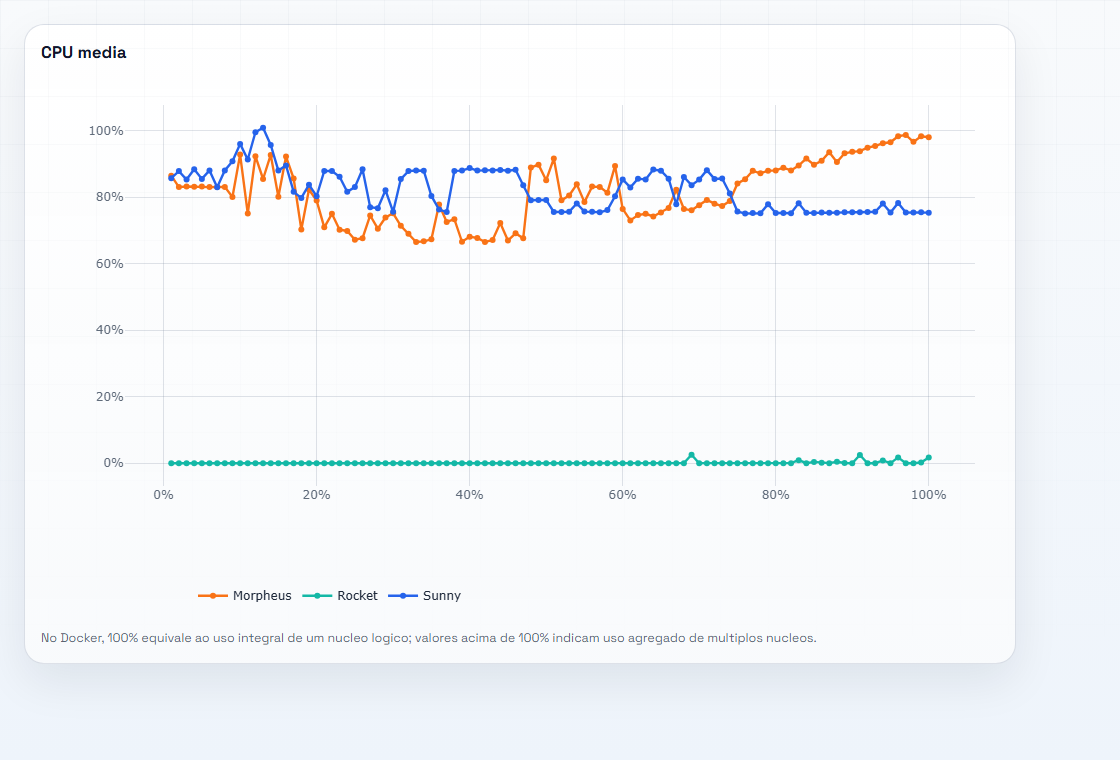
\includegraphics[width=0.9\linewidth,keepaspectratio]{figuras/benchmark/Figura_49_dashboard_cpu_i3_taxa_crossover.png}
\fonteautores
\notaacademica{100\% de CPU representa aproximadamente o uso integral de um núcleo lógico na telemetria do Docker; valores superiores indicam uso agregado de múltiplos núcleos.}
\end{figure}

\begin{figure}[H]
\centering
\caption{Uso médio de RAM na variação da taxa de crossover no cenário i3, conforme visualização filtrada no Dashboard IGRIS}
\label{fig:benchmark-ram-i3-crossover}
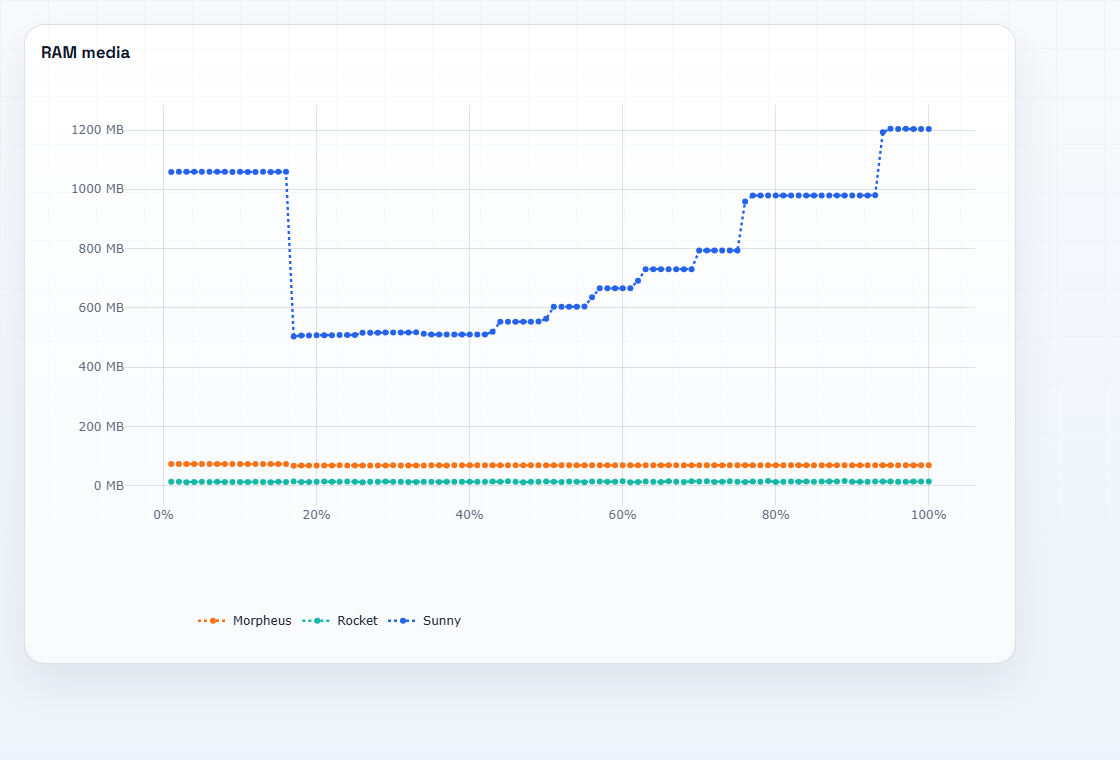
\includegraphics[width=0.9\linewidth,keepaspectratio]{figuras/benchmark/Figura_50_dashboard_ram_i3_taxa_crossover.png}
\fonteautores
\end{figure}

Essa diferença de memória pode estar relacionada ao conjunto formado por arquitetura do microsserviço, runtime utilizado, framework adotado, estrutura de dados e gerenciamento interno de memória. No caso do Sunny, a execução sobre o ecossistema Java pode contribuir para maior ocupação de memória. No caso do Rocket, a implementação em Go, a organização dos índices e o uso de estruturas mais compactas podem ter contribuído para o menor consumo. Entretanto, como os relatórios não apresentam profiling de heap, logs de Garbage Collector ou rastreamento detalhado de alocação, essa explicação deve ser tratada como hipótese, e não como conclusão definitiva.

No comportamento evolutivo, o Morpheus apresentou média de 191,38 gerações, o Rocket apresentou média de 191,52 gerações e o Sunny apresentou média de 945 gerações. Além disso, o Morpheus acionou parada antecipada em 8.979 execuções, o Rocket em 8.980 execuções e o Sunny não apresentou ocorrências de early stop. Esse dado indica que, na maior parte das execuções, Morpheus e Rocket encontraram um ponto de estabilização antes do limite máximo de gerações.

O erro médio foi igual para os três algoritmos, com valor de 3,00. Já o melhor score foi igual entre Morpheus e Rocket, com -29.574, e ligeiramente inferior no Sunny, com -29.640. Como valores menos negativos representam melhor avaliação relativa, Morpheus e Rocket tiveram pequena vantagem nessa métrica. No entanto, a diferença absoluta entre os scores é baixa em relação às penalidades utilizadas pela função \textit{fitness}, o que exige cautela na interpretação.

Diante dos resultados do cenário i3, o Rocket apresentou o melhor desempenho operacional, principalmente em tempo de resposta e consumo de memória. O Morpheus permaneceu superior ao Sunny nas métricas operacionais, enquanto o Sunny manteve taxa de sucesso total, mas exigiu mais memória e executou mais gerações sem apresentar redução no erro médio final.
